\documentclass[compress]{beamer}

\usepackage[english]{babel}
\usepackage{pgfplots}     % para mostrar el histograma
\usepackage{ragged2e}     % Para justificar en beamer; usar \justifying
\usepackage{lmodern}      % Corrige el error al imprimir >>
\usepackage[T1]{fontenc}  % Corrige el error al imprimir <> y otros

\usetheme{Nord}
% \usetheme[style=light]{Nord}

\AtBeginSection[]
{
  \begin{frame}[c,noframenumbering,plain]
    \tableofcontents[sectionstyle=show/hide,subsectionstyle=show/show/hide]
  \end{frame}
}


% Portada
\title{Analizador Léxico de C creado con Flex}
\subtitle{Instituto Tecnológico de Costa Rica \\Compiladores e Intérpretes \\Semestre II 2020}
\author{Ronald Herrera Gámez}
\date{\today}

\begin{document}

\begin{frame}[plain,noframenumbering]
  \maketitle
\end{frame}

% Descripción de Scanning
\begin{frame}{Proceso de Scanning}

    \justifying
    Consiste en determinar las diferentes unidades elementales de un programa fuente, es decir, identifica los distintos lexemas de un lenguaje. 
    Para este proceso, el scanner busca patrones dentro del fuente que cumplan con instrucciones, operadores, identificadores, constantes, entre 
    otros, del lenguaje que se escanea.
    
    \begin{figure}
        \centering
        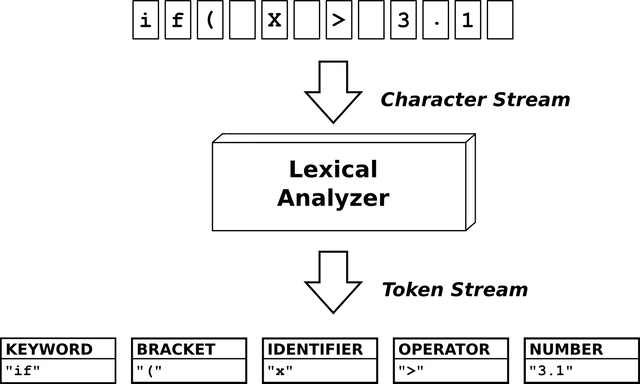
\includegraphics[scale=1.2]{images/scanning.png}
    \end{figure}

\end{frame}

% Descripción de Flex
\begin{frame}{Flex (Fast Lexical Analyzer)}
    \justifying
    Flex es una herramienta para generar analizadores léxicos basados en la teoría de autómatas finitos. Para ello, se crea la descripción del 
    escáner en forma de pares de expresiones regulares y código C, llamados reglas. Flex genera un archivo fuente en C llamado "lex.yy.c" que 
    se puede compilar y vincular para producir un ejecutable. Este ejecutable analiza su entrada en busca de ocurrencias de texto que coinciden 
    con las expresiones regulares para cada regla y siempre que encuentra una coincidencia, ejecuta el código C correspondiente.

    \begin{figure}
        \centering
        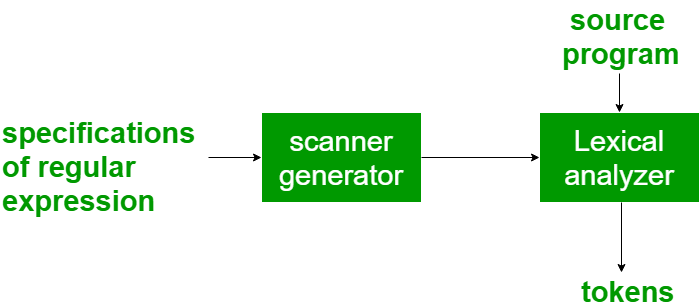
\includegraphics[scale=0.3]{images/flex.png}
    \end{figure}
    
\end{frame}

\begin{frame}{Código Después Del Preproceso}
\justifying\centering
\huge
    \textcolor{lime}{\textbf{TOKENS:}} \\ 
\small
    \textcolor{cyan}{\textbf{\\KEYWORD}}
    \textcolor{white}{\textbf{\\IDENTIFIER}}
    \textcolor{green}{\textbf{\\LITERAL}}
    \textcolor{yellow}{\textbf{\\OPERATOR}}
    \textcolor{magenta}{\textbf{\\PUNTUACTOR}}
    \textcolor{gray}{\textbf{\\COMMENT}}
    \textcolor{red}{\textbf{\\LEXICALERROR}}
    \textcolor{orange}{\textbf{\\PREPROCESSOR}}
    
\end{frame}

% Codigo generado por desde C: histograma y codigo
\justifying \small 

\textcolor{orange}{\#include <stdio.h>} 
\textcolor{gray}{/* Hello 
 * World program
 **/} 
\textcolor{cyan}{void} 
\textcolor{white}{main} 
\textcolor{magenta}{(} 
\textcolor{magenta}{)} 
\textcolor{magenta}{\{} 
\textcolor{gray}{// declara una variable "asd"*/} 
\textcolor{cyan}{int} 
\textcolor{white}{d} 
\textcolor{yellow}{=} 
\textcolor{green}{-.5e-1} 
\textcolor{yellow}{*} 
\textcolor{green}{521} 
\textcolor{magenta}{;} 
\textcolor{white}{printf} 
\textcolor{magenta}{(} 
\textcolor{green}{"resultado: \%d"} 
\textcolor{magenta}{,} 
\textcolor{white}{d} 
\textcolor{magenta}{)} 
\textcolor{magenta}{;} 
\textcolor{gray}{/*hello\textbackslash */} 
\textcolor{white}{printf} 
\textcolor{magenta}{(} 
\textcolor{green}{"ERROR AL COMPILAR LA EXPRESION (expResidencial)\textbackslash n"} 
\textcolor{magenta}{)} 
\textcolor{magenta}{;} 
\textcolor{cyan}{return} 
\textcolor{green}{0} 
\textcolor{magenta}{;} 
\textcolor{magenta}{\}} 
\textcolor{cyan}{if} 
\textcolor{magenta}{(} 
\textcolor{white}{L} 
\textcolor{yellow}{==} 
\textcolor{green}{4} 
\textcolor{magenta}{)} 
\textcolor{cyan}{if} 
\textcolor{magenta}{(} 
\textcolor{white}{F} 
\textcolor{yellow}{<} 
\textcolor{white}{l} 
\textcolor{green}{+18} 
\textcolor{magenta}{)} 
\textcolor{white}{a} 
\textcolor{yellow}{=} 
\textcolor{green}{6990400} 
\textcolor{magenta}{;} 
\textcolor{cyan}{else} 
\textcolor{cyan}{if} 
\textcolor{magenta}{(} 
\textcolor{white}{l} 
\textcolor{yellow}{>} 
\textcolor{white}{F} 
\textcolor{green}{-19} 
\textcolor{magenta}{)} 
\textcolor{white}{b} 
\textcolor{yellow}{*=} 
\textcolor{green}{0.7} 
\textcolor{magenta}{;} 
\textcolor{cyan}{if} 
\textcolor{magenta}{(} 
\textcolor{white}{L} 
\textcolor{yellow}{==} 
\textcolor{green}{3} 
\textcolor{magenta}{)} 
\textcolor{magenta}{\{} 
\textcolor{cyan}{if} 
\textcolor{magenta}{(} 
\textcolor{magenta}{(} 
\textcolor{white}{i} 
\textcolor{green}{-1} 
\textcolor{yellow}{\&} 
\textcolor{green}{15} 
\textcolor{magenta}{)} 
\textcolor{yellow}{<} 
\textcolor{green}{14} 
\textcolor{yellow}{\&} 
\textcolor{magenta}{(} 
\textcolor{white}{F} 
\textcolor{green}{-1} 
\textcolor{yellow}{\&} 
\textcolor{green}{15} 
\textcolor{magenta}{)} 
\textcolor{yellow}{<} 
\textcolor{green}{14} 
\textcolor{yellow}{\&} 
\textcolor{yellow}{!} 
\textcolor{magenta}{(} 
\textcolor{white}{F} 
\textcolor{yellow}{\&} 
\textcolor{green}{16} 
\textcolor{magenta}{)} 
\textcolor{magenta}{)} 
\textcolor{magenta}{\{} 
\textcolor{white}{a} 
\textcolor{yellow}{=} 
\textcolor{green}{12359778} 
\textcolor{magenta}{;} 
\textcolor{white}{\_} 
\textcolor{yellow}{=} 
\textcolor{green}{7} 
\textcolor{yellow}{-} 
\textcolor{white}{i} 
\textcolor{magenta}{;} 
\textcolor{white}{k} 
\textcolor{yellow}{=} 
\textcolor{green}{7} 
\textcolor{yellow}{-} 
\textcolor{white}{F} 
\textcolor{yellow}{\%} 
\textcolor{green}{16} 
\textcolor{magenta}{;} 
\textcolor{white}{\_} 
\textcolor{yellow}{\textasciicircum =} 
\textcolor{white}{\_} 
\textcolor{yellow}{>>} 
\textcolor{green}{31} 
\textcolor{magenta}{;} 
\textcolor{white}{k} 
\textcolor{yellow}{\textasciicircum =} 
\textcolor{white}{k} 
\textcolor{yellow}{>>} 
\textcolor{green}{31} 
\textcolor{magenta}{;} 
\textcolor{white}{b} 
\textcolor{yellow}{=} 
\textcolor{green}{196} 
\textcolor{yellow}{-} 
\textcolor{white}{R} 
\textcolor{yellow}{\%} 
\textcolor{green}{32} 
\textcolor{yellow}{+} 
\textcolor{magenta}{(} 
\textcolor{white}{k} 
\textcolor{yellow}{>} 
\textcolor{white}{\_} 
\textcolor{magenta}{?} 
\textcolor{white}{k} 
\textcolor{magenta}{:} 
\textcolor{white}{\_} 
\textcolor{magenta}{)} 
\textcolor{yellow}{\%} 
\textcolor{green}{3} 
\textcolor{yellow}{*} 
\textcolor{green}{42} 
\textcolor{magenta}{;} 
\textcolor{magenta}{\}} 
\textcolor{cyan}{else} 
\textcolor{magenta}{\{} 
\textcolor{white}{b} 
\textcolor{yellow}{*=} 
\textcolor{green}{1} 
\textcolor{yellow}{+} 
\textcolor{white}{R} 
\textcolor{yellow}{\%} 
\textcolor{green}{2} 
\textcolor{yellow}{*} 
\textcolor{magenta}{(} 
\textcolor{green}{.5} 
\textcolor{yellow}{-} 
\textcolor{magenta}{(} 
\textcolor{white}{i} 
\textcolor{yellow}{\&} 
\textcolor{green}{1} 
\textcolor{magenta}{)} 
\textcolor{magenta}{)} 
\textcolor{magenta}{;} 
\textcolor{magenta}{\}} 
\textcolor{magenta}{\}} 
\textcolor{white}{D} 
\textcolor{magenta}{[} 
\textcolor{white}{H} 
\textcolor{magenta}{]} 
\textcolor{yellow}{=} 
\textcolor{magenta}{(} 
\textcolor{white}{a} 
\textcolor{yellow}{\&} 
\textcolor{green}{16711935} 
\textcolor{yellow}{|} 
\textcolor{magenta}{(} 
\textcolor{white}{a} 
\textcolor{yellow}{\&} 
\textcolor{green}{65280} 
\textcolor{magenta}{)} 
\textcolor{yellow}{<<} 
\textcolor{green}{24} 
\textcolor{magenta}{)} 
\textcolor{yellow}{*} 
\textcolor{magenta}{(} 
\textcolor{white}{b} 
\textcolor{yellow}{>>} 
\textcolor{magenta}{(} 
\textcolor{white}{F} 
\textcolor{yellow}{>>} 
\textcolor{green}{5} 
\textcolor{magenta}{)} 
\textcolor{magenta}{)} 
\textcolor{yellow}{>>} 
\textcolor{green}{8} 
\textcolor{yellow}{\&} 
\textcolor{green}{0} 
\textcolor{white}{xff00ff00ff} 
\textcolor{magenta}{;} 
\textcolor{magenta}{\}} 
\textcolor{magenta}{\}} 
\textcolor{magenta}{\}} 
\textcolor{magenta}{\}} 
\textcolor{magenta}{\}} 




\begin{frame}{Histograma Tokens Usados} 
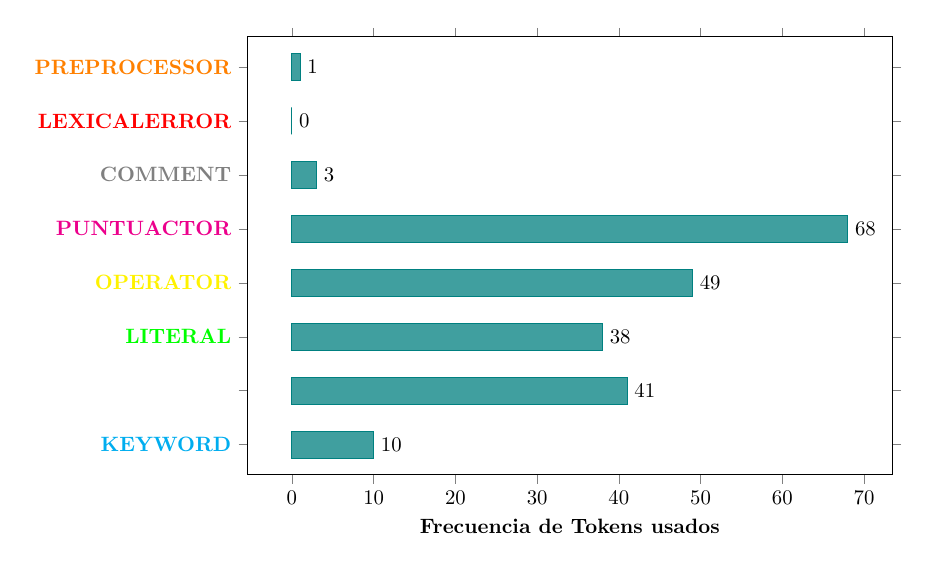
\begin{tikzpicture}[scale=0.75] % tamaño 
\begin{axis}[xbar,tick align=outside, 
    width=12.5cm,       % largo 
    height=9cm,       % altura 
    bar width={13pt},   % grosor linea 
    enlargelimits=0.08, % cercania a linea 
    nodes near coords, 
    nodes near coords align=horizontal, 
    point meta=x * 1, % The displayed number. 
    xlabel=\textbf{Frecuencia de Tokens usados}, 
    ytick={0,...,7}, 
    yticklabels={ 
        \textcolor{cyan}{\textbf{KEYWORD}},         % POSITION 0 
        \textcolor{white}{\textbf{IDENTIFIER}},     % POSITION 1 
        \textcolor{green}{\textbf{LITERAL}},        % POSITION 2 
        \textcolor{yellow}{\textbf{OPERATOR}},      % POSITION 3 
        \textcolor{magenta}{\textbf{PUNTUACTOR}},   % POSITION 4 
        \textcolor{gray}{\textbf{COMMENT}},         % POSITION 5 
        \textcolor{red}{\textbf{LEXICALERROR}},     % POSITION 6 
        \textcolor{orange}{\textbf{PREPROCESSOR}}   % POSITION 7 
    }] 
\addplot 
[draw=teal,fill=teal!75] 
coordinates {(10,0) (41,1) (38,2) (49,3) (68,4) (3,5) (0,6) (1,7)}; 
\end{axis}
\end{tikzpicture}
\end{frame}


\end{document}
